%%%%%%%%%%%%%%%%%%%%%%%%%%%%%%%%%%%%%%%%%%%%%%%%%%%%%%%%%%%%%%%%%%%%%%%%%%%%%%%%%
%
% Purpose:  Verification part of V&V for the NED model
%
% 
%
%%%%%%%%%%%%%%%%%%%%%%%%%%%%%%%%%%%%%%%%%%%%%%%%%%%%%%%%%%%%%%%%%%%%%%%%%%%%%%%%

% \section{Verification}

%%% code imported from old template structure
\subsection{Inspection of Modeling Requirements}


\inspection{State Encapsulation}\label{inspect:NED}
 The \NEDDesc\ is capable of outputting data as desired, as demonstrated in simulations located at \textit{derived\_state/verif/SIM\_NED/}, thereby satisfying
 requirement \ref{reqt:NED} at the inspection level.

\inspection{Frame Generation}\label{inspect:NED_frame}
 The \NEDDesc\ is capable of generating a reference frame, as demonstrated in simulations located at \textit{derived\_state/verif/SIM\_NED/}, thereby satisfying
 requirement \ref{reqt:NED_frame} at the inspection level.


\subsection{Verification of Model}

 For testing the \NEDDesc, a simulation of two vehicles was established in which the two vehicles are separated by 1 degree on a common orbital trajectory. Both vehicles generate a North-East-Down reference frame, and the relative state of the other vehicle is calculated for both.

\test{Verification of \NEDDesc\ Output Data for Generic Orbits}\label{test:NED}

\begin{description}
\item{Purpose:}\newline
To demonstrate that the data output by the \NEDDesc\ provides meaningful data.

\item{Requirements:}\newline
Satisfactory conclusion of this test satisfies requirement \ref{reqt:NED}

\item{Procedure:}\newline
The data from the North-East-Down output was compared against that from a Planetary Derived State for an identical orbit.  Polar, inclined, and equatorial orbital characteristics were each tested.

\item{Predictions:}
The state output from this simulation should match that from a Planetary Derived State, which has been verified independently in the \textref{PlanetaryDerivedState Verification Section}{ch:planetaryvv}.

\item{Results:}
There appeared to be no, or negligible, differences between the two states. 
\end{description}



\test{Verification of the reference frame orientation}\label{test:NED_frame}
\begin{description}
\item{Purpose:}\newline
To demonstrate that the reference frame generated by the \NEDDesc\ is oriented along the intended axes.

\item{Requirements:}\newline
Satisfactory conclusion of this test satisfies requirement \ref{reqt:NED_frame}

\item{Procedure:}\newline
The relative state data between the two vehicles was compared against theoretical prediction for consistency for polar, inclined, and equatorial orbital characteristics.

\item{Predictions:}
\begin{enumerate}
 \item {Polar orbit.}  
  \begin{enumerate}
   \item{North.} The lead vehicle should be North of the trailing vehicle while latitude is increasing, and South of the trailing vehicle while the latitude is decreasing.  The transition should be sharp, though not coincident between the two frames; as the vehicles cross the pole, the state of the trailing vehicle in the NED frame associated with the lead vehicle should transition first, resulting in a short time when both vehicles are north (or south) of each other. 
   \item {East.}  The relative states should show zero East component in their respective positions.
   \item {Down.}  Because the NED states are rectilinear, both vehicles should be represented as having a state with a positive down component at all times.  See Figure~\ref{fig:nedrectilinear} for a partial illustration of this counter-intuitive phenomenon.  The behavior is also dependent upon the planetary geometry:
   \begin{itemize}
    \item {Spherical.}  The Down component should be constant, at a value equal to $r - r \cos \Delta \theta$.  For these simulations, this value equates to $1.03 km$. 
    \item {Elliptical.} The Down component should oscillate.  In these simulations, the orbit is approximately circular, whereas the definition of \textit{down} is elliptical.  As the vehicles leave the equator, the trailing vehicle should be significantly further below the leading vehicle than the leading vehicle below the trailing vehicle.  As the vehicles approach the poles, the two values should equalize to $1.03 km$, due to symmetry, then drift apart again heading back to the equator; this time, however, the leading vehicle should have the larger down component.  As the vehicles approach the equator again, the values should again equalize, again due to symmetry.  An exaggerated illustration of this is shown in Figure~\ref{fig:nedellipticalrectilinear}.

\begin{figure}[!ht]
\begin{center}
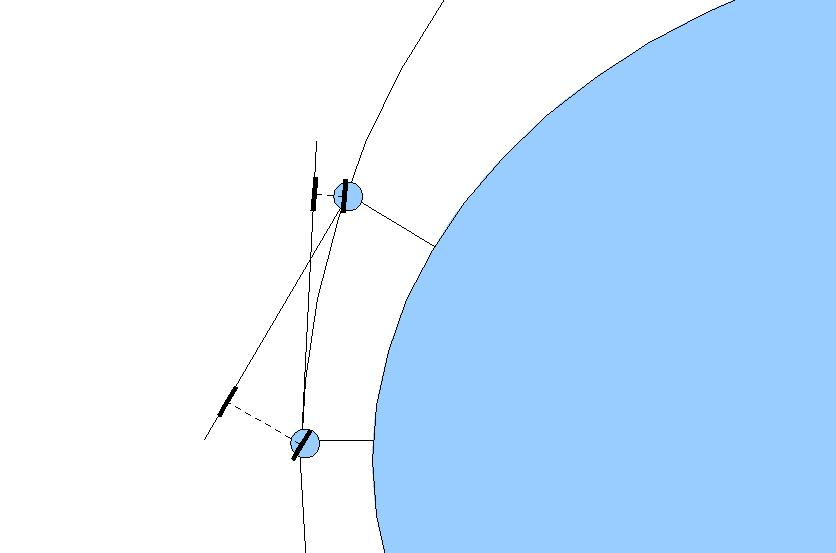
\includegraphics[width=5in]{figures/ned_elliptical_rectilinear.jpg}
\caption{The effect of the difference between the curvature of an orbit and that of the reference ellipse on the relative state using rectilinear coordinates.  The vehicle closer to the equator will exhibit a larger down component in its state than the vehicle farther from the equator.}
\label{fig:nedellipticalrectilinear}
\end{center}
\end{figure}

   \end{itemize}
  \end{enumerate}
 \item {Inclined orbit.}
  \begin{enumerate}
   \item{North.}  As for the polar orbit, the lead vehicle should be North of the trailing vehicle while latitude is increasing, and South of the trailing vehicle while the latitude is decreasing.  Conversely, the transitions at the poles will differ from those observed for the polar orbit; for the inclined orbit, the North component of the relative state should be oscillatory, and ninety degrees out-of-phase from the latitude measurement (so that the North component of the relative state reaches an extremum when the vehicles are at the equator, and goes to zero when the vehicles are at their extreme latitudes).  
   \item {East.}  The lead vehicle should always be East of the trailing vehicle, and the trailing vehicle negative-East of the lead vehicle.
   \item {Down.} By the same argument put forth for the polar orbit, both vehicles should be represented as having a state with a positive down component at all times, constant for spherical geometry and oscillating (though with smaller magnitude due to the variation of the curvature being less significant on an inclined orbit) for the elliptical geometry.  
  \end{enumerate}


 \item {Equatorial orbit.}  
  \begin{enumerate}
   \item{North.} Both relative states should have zero North component.
   \item {East.} The lead vehicle should always be East of the trailing vehicle, and the trailing vehicle negative-East of the lead vehicle.
   \item {Down.} By the same argument put forth for the polar orbit, both vehicles should be represented as having a state with a positive down component at all times, but now be constant for both spherical and elliptical geometries.  
  \end{enumerate}




\end{enumerate}


\item{Results:}
\begin{enumerate}
 \item {Polar orbit.} \ \newline
   The results were mostly as expected.  Figures~\ref{fig:nedpolarell} and \ref{fig:nedpolarellzoom} show the results from the elliptical-geometry reference frame, and Figure~\ref{fig:nedpolarsph} the results from the spherical-geometry reference frame.
  \begin{enumerate}
   \item{North.} The instantaneous switch is seen at polar crossings, with the offset between the two states illustrated better in Figure~\ref{fig:nedpolarellzoom}.  This is at a South pole crossing, and it is clear that the trailing vehicle first transitions to being South of the leading vehicle, then the leading vehicle transitions to being North of the trailing vehicle.
   \item {East.}  The East component is not uniformly zero, it has some instantaneous spikes in its value.  This is attributed to numerical error; those spikes all occur as the vehicles transit the poles, where North and East are not well defined.  
   \item {Down.} For the spherical geometry, the down component shows some oscillation, but that oscillation has magnitude less than $1 cm$, and the mean has the expected value of $1.03 km$.  For the elliptical geometry, the oscillation can clearly be seen.  Figure~\ref{fig:nedpolarellzoom} shows the oscillation from equator heading North (trailing vehicle has larger down component), through the pole at about $1400 s$, then back South to the equator again at approximately $2800 s$.
  \end{enumerate}

\begin{figure}[!ht]
\begin{center}
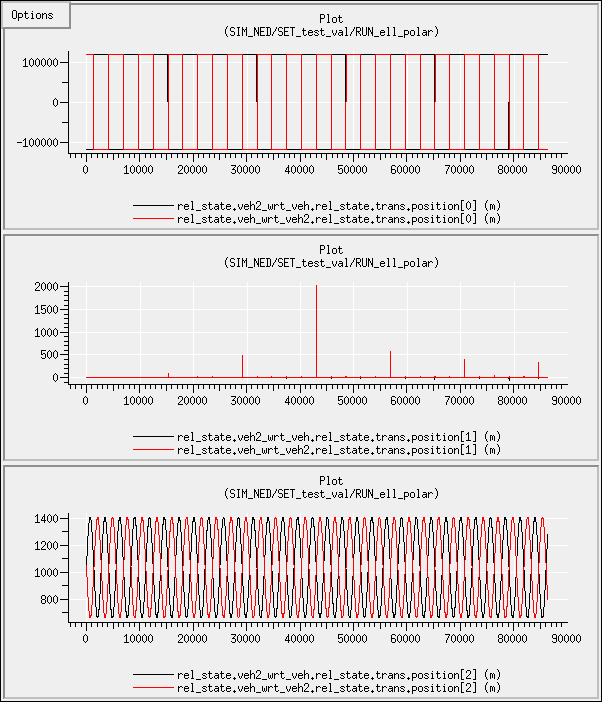
\includegraphics[width=5in]{figures/ned_polar_ell.jpg}
\caption{The relative states for a polar orbit, with elliptical geometry used to define the reference frame.}
\label{fig:nedpolarell}
\end{center}
\end{figure}

\begin{figure}[!ht]
\begin{center}
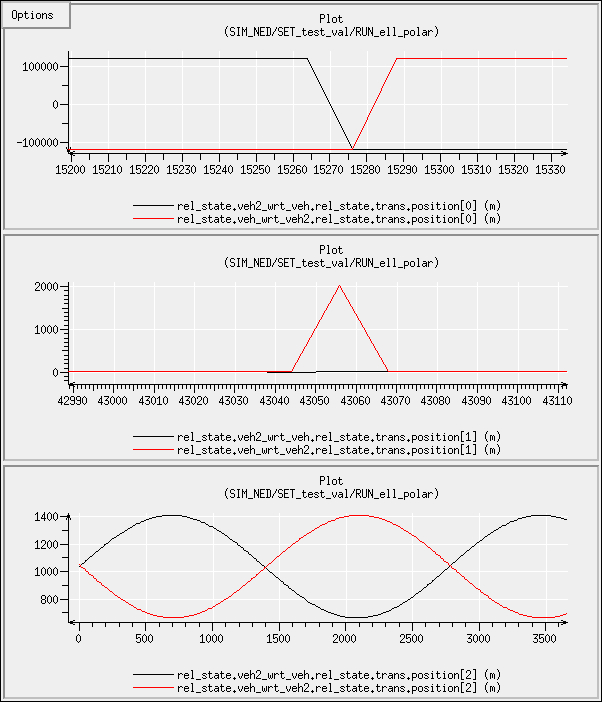
\includegraphics[width=5in]{figures/ned_polar_ell_zoom.jpg}
\caption{The relative states for a polar orbit, with elliptical geometry used to define the reference frame, zoomed in to locations of interest.}
\label{fig:nedpolarellzoom}
\end{center}
\end{figure}

\begin{figure}[!ht]
\begin{center}
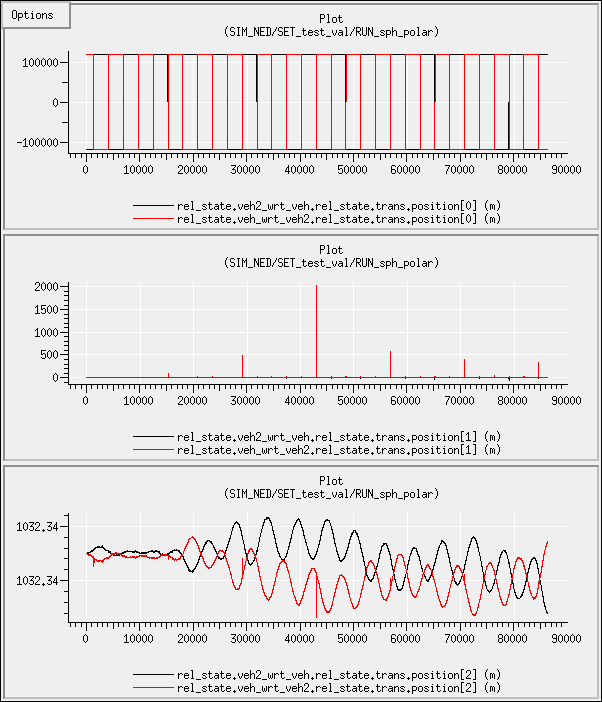
\includegraphics[width=5in]{figures/ned_polar_sph.jpg}
\caption{The relative states for a polar orbit, with spherical geometry used to define the reference frame.}
\label{fig:nedpolarsph}
\end{center}
\end{figure}

\clearpage

\item {Inclined Orbit.} \ \newline
  The results match with expectation.  Figure~\ref{fig:nedincsph} shows the North and East components with the latitude history.  The Down components had a similar oscillation to those seen in the polar orbit and are not shown. A small difference exists of order meters between the North components of the spherical and elliptical geometries, East shows no dependence on geometry, and Down shows a large dependence, as it did in the polar orbit.


\begin{figure}[!ht]
\begin{center}
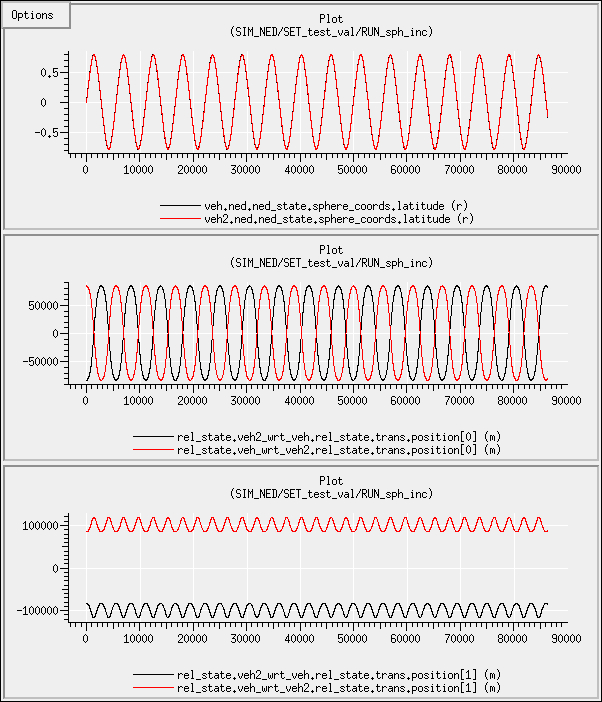
\includegraphics[width=5in]{figures/ned_inc_sph.jpg}
\caption{The variation with time of latitude and of the North and East components of the relative states for an orbit inclined at 45 degrees, with spherical geometry used to define the reference frame.}
\label{fig:nedincsph}
\end{center}
\end{figure}

\clearpage

\item{Equatorial Orbit.}\ \newline
  The results match with expectation.  Figure~\ref{fig:nedequsph} shows the state components; there was no noticeable difference between the spherical and elliptical geometries.
\end{enumerate}

\begin{figure}[!ht]
\begin{center}
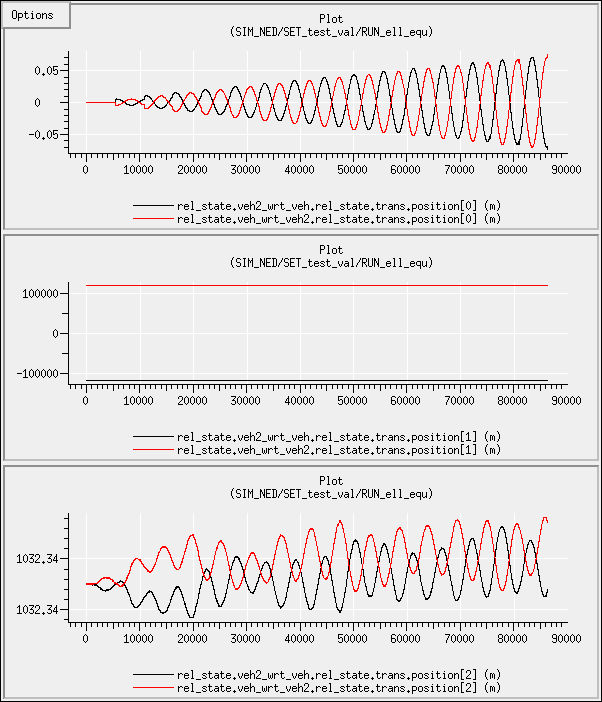
\includegraphics[width=5in]{figures/ned_equ_sph.jpg}
\caption{The relative states for an equatorial orbit with spherical geometry used to define the reference frame.}
\label{fig:nedequsph}
\end{center}
\end{figure}

\end{description}



